\documentclass[10pt,conference]{IEEEtran}
\IEEEoverridecommandlockouts

\usepackage{cite}
\usepackage{amsmath,amssymb,amsfonts}
\usepackage{algorithmic}
\usepackage{graphicx}
\usepackage{textcomp}
\usepackage{xcolor}
\usepackage{booktabs}
\usepackage{multirow}
\usepackage{url}

\def\BibTeX{{\rm B\kern-.05em{\sc i\kern-.025em b}\kern-.08em
    T\kern-.1667em\lower.7ex\hbox{E}\kern-.125emX}}

\begin{document}

\title{DecisionSphere: A Scenario-Based Strategic Planning and Risk Evaluation Platform}

\author{\IEEEauthorblockN{P Naga Venkata Kushal\IEEEauthorrefmark{1}, P Manjunatha Kumar Tejas\IEEEauthorrefmark{2}, Jeswanth Reddy Sagabala\IEEEauthorrefmark{3}, and Suresh A\IEEEauthorrefmark{4}}
\IEEEauthorblockA{School of Computer Science and Engineering (SCOPE)\\
Vellore Institute of Technology, Vellore, Tamil Nadu, India\\
Email: \IEEEauthorrefmark{1}kushal.pnv2023@vitstudent.ac.in,
\IEEEauthorrefmark{2}tejas.pmk2023@vitstudent.ac.in,
\IEEEauthorrefmark{3}jeswanth.rs2023@vitstudent.ac.in,
\IEEEauthorrefmark{4}suresh.a@vit.ac.in}
}

\maketitle

\begin{abstract}
Strategic business decisions inherently trigger cascading cross-domain consequences across enterprise operations. However, contemporary enterprise decision support systems operate within isolated operational silos: demand forecasting is restricted to sales, logistics delivery risk is isolated in fulfillment, and employee attrition is confined to human resources. Consequently, commercial initiatives such as promotional expansions frequently induce unbuffered operational strains, resulting in carrier delays, workforce burnout, and severe bottom-line margin collapse. This paper introduces \textbf{DecisionSphere}, an integrated, scenario-based strategic planning and risk evaluation platform. DecisionSphere couples three independently trained, calibrated machine learning models across retail demand forecasting (Rossmann Store Sales), logistics delivery risk classification (DataCo Supply Chain), and employee attrition risk (IBM HR Analytics) into a unified 13-stage linear execution pipeline. Downstream operational impacts are propagated via deterministic parameterized coupling equations, feeding a transparent managerial accounting engine and a rule-grounded recommendation synthesizer. We enforce a strict six-tier epistemic hierarchy, preventing non-causal machine learning predictions from being conflated with empirical fact or causal certainty. Evaluated on an authoritative enterprise scenario ($+15.0\%$ demand shock, active promotional push, and $40.0\%$ mandatory overtime), DecisionSphere demonstrates how a commercial surge of $+28,551.04$ units generates $+\$26,710.78$ in realized revenue yet triggers $+\$469,188.49$ in logistics delay penalties and $+\$184,212.00$ in labor disruption costs, collapsing net operating profit by $-\$642,716.18$ and automatically triggering an objective restructuring rejection (\texttt{REJECT\_RESTRUCTURE}, Composite Risk Score 37.48). The platform is implemented as a full-stack system with a FastAPI backend, React/Next.js frontend, 236 verified unit tests, and 16 reproducible research notebooks.
\end{abstract}

\begin{IEEEkeywords}
Decision Intelligence, Strategic Planning, Cross-Domain Simulation, Demand Forecasting, Supply Chain Risk, Workforce Attrition, Explainable AI, Probability Calibration.
\end{IEEEkeywords}

\section{Introduction}

\subsection{Background and Motivation}
In modern enterprises, operational decision-making relies heavily on predictive machine learning (ML) systems. However, these analytical assets exist almost universally within isolated functional departments \cite{pratt2019decision}. Commercial marketing teams utilize time-series forecasting models to maximize sales volume; fulfillment logistics centers deploy classification algorithms to track shipping exceptions; and human resource departments evaluate attrition risk models to retain key talent.

While functional specialization optimizes local departmental objectives, strategic business interventions inherently produce cascading systemic ripples that cross departmental boundaries \cite{lee1997bullwhip}. For example, an aggressive promotional campaign designed to elevate quarterly top-line revenue induces immediate upstream and downstream consequences:
\begin{enumerate}
    \item Commercial demand surges, expanding distribution requirements.
    \item Warehouse dispatch lines experience volume strain, elevating carrier late delivery probabilities.
    \item Operations imposes mandatory overtime on fulfillment personnel to mitigate logistics delays.
    \item Chronic overtime elevates workplace stress and accelerates voluntary employee turnover \cite{maslach2001burnout}.
    \item Contractual delay penalties and premium overtime wages eradicate gross margins, transforming a projected commercial success into an enterprise financial deficit.
\end{enumerate}

\subsection{Limitations of Current Approaches}
Traditional Business Intelligence (BI) dashboards (e.g., Tableau, PowerBI) provide retrospective descriptive metrics (what occurred in the past) rather than counterfactual scenario simulation (what will occur if policies change). Conversely, emerging Generative AI decision tools rely on large language models (LLMs) that frequently hallucinate numerical accounting values, rendering them unacceptable for capital allocation. 

Furthermore, point machine learning models deployed in production are rarely calibrated probabilistically \cite{guo2017calibration}. Uncalibrated classifiers output arbitrary decision scores rather than true empirical probabilities, undermining any financial accounting equations that depend on risk-weighted expected loss.

\subsection{Contributions}
This paper presents DecisionSphere, addressing the fragmentation of enterprise decision support. Our core contributions are:
\begin{enumerate}
    \item \textbf{Integrated Multi-Domain Architecture:} Unification of retail demand forecasting, supply chain late delivery classification, and workforce attrition risk into a single, cohesive 13-stage execution pipeline.
    \item \textbf{Strict Epistemic Demarcation:} Explicit separation of variables across six epistemic tiers (Observed, Predicted, Assumed, Propagated, Calculated, Recommended), establishing scientific boundaries against unwarranted causal assertions \cite{shmueli2010explain}.
    \item \textbf{Deterministic Decision Synthesis:} A transparent managerial accounting and lexicographic risk engine linking calibrated ML outputs to exact dollar profit-and-loss deltas without generative hallucinations.
    \item \textbf{Rigorous Verification and Reproducibility:} A fully containerized platform validated across 236 automated tests, 16 executable research notebooks, cryptographic SHA-256 model integrity checks, and a production-grade web interface.
\end{enumerate}

\section{Related Work}

\subsection{Decision Intelligence and Counterfactual Simulation}
Decision Intelligence (DI) emerged to bridge the gap between predictive machine learning algorithms and real-world organizational actions \cite{pratt2019decision}. While classical operations research relies on closed-form mixed-integer linear programming (MILP), modern enterprise environments require data-driven predictive models capable of processing high-dimensional non-linear features. However, existing DI platforms remain largely proprietary or fail to incorporate transparent managerial accounting.

\subsection{Predictive Machine Learning in Enterprise Domains}
Demand forecasting has evolved from classical seasonal ARIMA architectures to gradient-boosted decision trees \cite{chen2016xgboost}, which capture complex non-linear calendar and promotional interactions. In supply chain analytics, delay classification models frequently suffer from contemporaneous lookahead leakage—incorporating post-checkout transit milestones that inflate validation metrics but render models useless at order creation \cite{constante2019dataco}. In human capital analytics, employee attrition modeling is hindered by severe class imbalance and uncalibrated risk scoring \cite{guo2017calibration}.

\subsection{Explainable AI and Probability Calibration}
Explainable AI (XAI) is essential for executive trust. SHAP and TreeSHAP \cite{lundberg2017unified, lundberg2020treeshap} provide game-theoretically optimal, polynomial-time Shapley attributions for tree ensembles. However, high feature importance is frequently misinterpreted by business practitioners as causal influence. Furthermore, without probability calibration (e.g., Platt Scaling \cite{platt1999probabilistic}), predicted classification probabilities diverge from empirical frequencies, invalidating risk-weighted expected cost computations.

\section{Problem Formulation}

Let an enterprise operational scenario $S$ be formalized as a tuple:
\begin{equation}
S = \langle \mathbf{\theta}_{\text{scen}}, \mathbf{w}_{\text{policy}}, \mathbf{c}_{\text{cost}} \rangle
\end{equation}
where $\mathbf{\theta}_{\text{scen}} = [\Delta D, P, \Delta L, M_{\text{ship}}, \Delta O, \Delta W]$ represents user-defined scenario levers (demand shock percentage, promotional flag, lead-time offset, shipping mode, overtime adjustment, and wage hike); $\mathbf{w}_{\text{policy}} = [w_{\text{supply}}, w_{\text{workforce}}, w_{\text{demand}}]$ denotes the normalized policy weighting simplex ($\sum w_i = 1$); and $\mathbf{c}_{\text{cost}}$ represents baseline managerial accounting unit constants.

The decision problem requires evaluating scenario $S$ relative to empirical baseline $S_0$:
\begin{align}
\Delta \Pi(S) &= \Delta \text{Realized Revenue}(S) - \Delta \text{COGS}(S) \nonumber \\
&\quad - \Delta \text{Logistics Cost}(S) - \Delta \text{Labor Cost}(S) \\
\text{CRS}(S) &= \sum_{i \in \{\text{sup}, \text{wf}, \text{dem}\}} w_i \cdot \text{Strain}_i(S) \in [0, 100] \\
\text{Decision}(S) &\in \{\text{APPROVE}, \text{APPROVE\_COND}, \text{REJECT}, \text{CRIT\_REJECT}\}
\end{align}
The platform must compute $\Delta \Pi(S)$, $\text{CRS}(S)$, and synthesize rule-grounded strategic actions $\mathcal{A}(S)$ deterministically.

\section{Data and Experimental Setup}

\subsection{Benchmark Datasets}
DecisionSphere utilizes three standardized, peer-reviewed public benchmark datasets:
\begin{enumerate}
    \item \textbf{Retail Demand:} Rossmann Store Sales benchmark \cite{rossmann2015kaggle}, encompassing 1,115 retail pharmacy stores across 1,017,209 daily transactional observations.
    \item \textbf{Supply Chain Logistics:} DataCo Smart Supply Chain dataset \cite{constante2019dataco}, comprising 180,519 global order shipments spanning standard, first-class, and second-class fulfillment.
    \item \textbf{Workforce Human Capital:} IBM HR Analytics Employee Attrition benchmark \cite{ibm2017attrition}, containing 1,470 employee records across 35 demographic, compensation, and operational attributes.
\end{enumerate}

The empirical dimensions, target variables, and partition protocols across all three benchmark domains are summarized in Table~\ref{tab:datasets}.

\begin{table}[htbp]
\caption{Benchmark Dataset Summary and Partitioning Protocols}
\begin{center}
\begin{tabular}{lcccc}
\toprule
\textbf{Domain} & \textbf{Observations} & \textbf{Features} & \textbf{Target} & \textbf{Split Protocol} \\
\midrule
Demand & 1,017,209 & 18 & Sales (Units) & Chronological (2013--15) \\
Logistics & 180,519 & 24 & Late Risk (0/1) & Chronological Holdout \\
Workforce & 1,470 & 32 & Attrition (0/1) & Stratified Holdout (80/20) \\
\bottomrule
\end{tabular}
\label{tab:datasets}
\end{center}
\end{table}

\subsection{Anti-Leakage Engineering}
To guarantee scientific validity, strict anti-leakage invariants are enforced:
\begin{itemize}
    \item \textbf{Chronological Partitioning:} Retail demand is split strictly by date. Training encompasses 2013-01-01 through 2014-12-31; evaluation is conducted on the subsequent holdout period (2015-01-01 to 2015-07-31). Random shuffling is prohibited.
    \item \textbf{Order-Time Predictor Registry:} In logistics classification, all post-checkout transit milestones (\texttt{Actual shipping days}, carrier scan timestamps) are quarantined via an immutable \texttt{PROHIBITED\_LOOKAHEAD\_COLUMNS} registry. The model evaluates strictly order-time features.
    \item \textbf{Pre-Split Feature Encoding:} In workforce modeling, one-hot encoders, imputers, and standardizers are fitted strictly on the training partition prior to transforming holdout data.
\end{itemize}

\section{Predictive Modeling and Calibration}

\subsection{Retail Demand Forecasting}
We benchmark three model tiers: Naive Seasonal (Level 0), Ridge Linear Regression (Level 1), and an optimized XGBoost Regressor (Level 2) \cite{chen2016xgboost}. The XGBoost regressor minimizes root mean squared error across calendar lags ($t-1, t-7, t-14, t-28$), promotional indicators, and store competition metrics.
As shown in Table~\ref{tab:model_performance}, XGBoost reduces Weighted Absolute Percentage Error (WAPE) from $33.32\%$ (naive) to $8.12\%$.

\subsection{Supply Chain Late Delivery Risk}
Logistics delivery risk is modeled as binary classification predicting late arrival probability $\hat{P}_{\text{late}} \in [0, 1]$. An XGBoost classifier achieves $\text{ROC-AUC} = 0.7795$ and $\text{PR-AUC} = 0.8423$. 

Because raw tree ensemble margins yield uncalibrated probabilities, we apply Sigmoid (Platt) scaling \cite{platt1999probabilistic} on an independent validation set. Calibration reduces Expected Calibration Error (ECE) to $0.0142$ (Brier score $0.1807$). At the calibrated decision threshold $\tau^* = 0.17$, the classifier achieves $F_1 = 0.7224$ and $\text{Recall} = 1.0000$, ensuring comprehensive late delivery capture.

\subsection{Workforce Attrition Risk}
Employee turnover risk is evaluated under an 84:16 class imbalance. XGBoost achieves $\text{ROC-AUC} = 0.8045$ and $\text{PR-AUC} = 0.5030$. Sigmoid calibration compresses ECE to $0.0537$. At optimal threshold $\tau^* = 0.21$, the model yields $F_1 = 0.4706$, $\text{Recall} = 0.5556$, and $\text{Specificity} = 0.8432$.

\begin{table}[htbp]
\caption{Empirical Model Performance and Calibration Benchmarks}
\begin{center}
\begin{tabular}{llcccc}
\toprule
\textbf{Domain} & \textbf{Model} & \textbf{Primary Metric} & \textbf{ROC-AUC} & \textbf{ECE} & \textbf{Brier} \\
\midrule
Demand & Naive Seasonal & 33.32\% WAPE & --- & --- & --- \\
Demand & Ridge Regression & 11.98\% WAPE & --- & --- & --- \\
Demand & \textbf{XGBoost Regressor} & \textbf{8.12\% WAPE} & --- & --- & --- \\
\midrule
Supply Chain & Majority Class & 0.5000 AUC & 0.5000 & --- & 0.2730 \\
Supply Chain & Logistic Regression & 0.7520 AUC & 0.7520 & 0.0381 & 0.1920 \\
Supply Chain & \textbf{Calibrated XGBoost} & \textbf{0.7795 AUC} & \textbf{0.7795} & \textbf{0.0142} & \textbf{0.1807} \\
\midrule
Workforce & Class Ratio Naive & 0.1629 PR-AUC & 0.5000 & --- & 0.1360 \\
Workforce & Logistic Regression & 0.6190 PR-AUC & 0.8330 & 0.0712 & 0.1140 \\
Workforce & \textbf{Calibrated XGBoost} & \textbf{0.5030 PR-AUC} & \textbf{0.8045} & \textbf{0.0537} & \textbf{0.1086} \\
\bottomrule
\end{tabular}
\label{tab:model_performance}
\end{center}
\end{table}

\subsection{Explainability via TreeSHAP}
Pre-computed TreeSHAP attributions \cite{lundberg2020treeshap} reveal that commercial promotions (\texttt{Promo}, attribution $+0.412$) and day-of-week dominantly drive retail demand. In logistics, shipping mode and customer geographic region dominate delay probabilities. In workforce attrition, mandatory overtime (\texttt{OverTime}, attribution $+0.445$) and compensation stock tiers (\texttt{StockOptionLevel}, $+0.343$) represent the primary predictive contributors.

\section{Cross-Domain Scenario Propagation}

To simulate hypothetical scenarios without retraining frozen models, DecisionSphere implements parameterized operational coupling:
\begin{enumerate}
    \item \textbf{Demand Shock to Logistics Dispatch:} When commercial demand expands by $\Delta D$, operational order volume scales proportionally:
    \begin{equation}
    V_{\text{scen}} = V_{\text{base}} \times (1 + \Delta D)
    \end{equation}
    Fulfillment features (shipping class, scheduled days adjusted by $\Delta L$) are updated and passed to the logistics classifier to evaluate scenario late delivery probability $\hat{P}_{\text{late, scen}}$.
    \item \textbf{Operational Surge to Workforce Strain:} Unbuffered fulfillment expansion elevates required operational labor. Mandatory overtime scales:
    \begin{equation}
    \text{OT}_{\text{scen}} = \min(1.0, \text{OT}_{\text{base}} + \Delta O)
    \end{equation}
    When $\text{OT}_{\text{scen}} > 0.25$, the binary overtime indicator toggles to 1 in employee feature vectors, elevating predicted attrition risk $\hat{P}_{\text{attr, scen}}$.
\end{enumerate}

\section{Deterministic Managerial Accounting Engine}

All financial outcomes are calculated using closed-form deterministic accounting formulas:
\begin{align}
\Delta \text{Gross Rev} &= \Delta \text{Units} \times \bar{P} \quad (\bar{P} = \$1.00) \\
\Delta \text{Realized Rev} &= \Delta \text{Gross Rev} \times (1 - \hat{P}_{\text{late, scen}} \cdot c_{\text{loss}}) \\
\Delta \text{COGS} &= \Delta \text{Units} \times c_{\text{cogs}} \quad (c_{\text{cogs}} = \$0.56133) \\
\Delta \text{Logistics Cost} &= V_{\text{scen}} \cdot \hat{P}_{\text{late, scen}} \cdot c_{\text{pen}} - V_{\text{base}} \cdot \hat{P}_{\text{late, base}} \cdot c_{\text{pen}} \\
\Delta \text{Labor Cost} &= W \cdot \bar{S}_{\text{hr}} \cdot (\text{OT}_{\text{scen}} \cdot 1.5 - \text{OT}_{\text{base}}) \nonumber \\
&\quad + W \cdot (\hat{P}_{\text{attr, scen}} - \hat{P}_{\text{attr, base}}) \cdot c_{\text{rep}} \\
\Delta \Pi &= \Delta \text{Realized Rev} - \Delta \text{COGS} - \Delta \text{Logistics} - \Delta \text{Labor}
\end{align}
where $W$ is total workforce headcount, $\bar{S}_{\text{hr}}$ is baseline hourly wage, $c_{\text{pen}}$ is delay penalty (\$45/order), and $c_{\text{rep}}$ is employee replacement cost (\$15,000).

\section{Risk and Recommendation Engine}

\subsection{Composite Risk Score (CRS)}
Domain operational strains $S_{\text{sup}}, S_{\text{wf}}, S_{\text{dem}} \in [0, 100]$ are synthesized via policy simplex weights ($w_{\text{sup}}=0.40, w_{\text{wf}}=0.35, w_{\text{dem}}=0.25$):
\begin{equation}
\text{CRS} = 0.40 S_{\text{sup}} + 0.35 S_{\text{wf}} + 0.25 S_{\text{dem}}
\end{equation}

\subsection{Rule-Grounded Strategic Actions}
Seven deterministic policy rules govern scenario categorization and strategic action synthesis:
\begin{itemize}
    \item \textbf{RULE-01 (Supply Buffer):} If $\hat{P}_{\text{late}} \ge 0.60$, trigger secondary carrier buffers.
    \item \textbf{RULE-02 (Carrier Penalty):} If $\hat{P}_{\text{late}} \ge 0.75$ and shipping is express, enforce contractual carrier SLA penalties.
    \item \textbf{RULE-03 (Overtime Cap):} If $\hat{P}_{\text{attr}} \ge 0.25$ or $\text{OT} \ge 0.30$, cap overtime and mandate retention incentives.
    \item \textbf{RULE-04 (Margin Erosion):} If $\Delta \Pi < 0$ and $\Delta D > 0$, trigger critical alert to rescale promotional intensity.
    \item \textbf{RULE-05 (Inventory Rebalance):} If stockout risk $\ge 0.40$, expedite safety stock replenishment.
    \item \textbf{RULE-06 (Circuit Breaker):} If $\text{CRS} \ge 75.0$, halt scenario implementation.
    \item \textbf{RULE-07 (Expansion Greenlight):} If $\Delta \Pi \ge 0$ and $\text{CRS} < 30.0$, authorize execution.
\end{itemize}

\section{System Architecture and Implementation}

As illustrated in Fig.~\ref{fig:arch}, DecisionSphere is engineered as a decoupled modern web platform:
\begin{itemize}
    \item \textbf{Analytical Core (\texttt{src/}, \texttt{models/}):} Pure Python analytical modules and frozen serialized estimators (\texttt{.joblib}), governed by cryptographic SHA-256 integrity checks (Gate H).
    \item \textbf{Backend REST API (\texttt{backend/}):} High-performance asynchronous FastAPI service serving Pydantic v2 validated endpoints for simulations, scenarios, sensitivity sweeps, and health monitoring.
    \item \textbf{Frontend User Interface (\texttt{frontend/}):} Single-page application built in Next.js 15, React 19, TypeScript, and Tailwind CSS, featuring progressive disclosure and interactive waterfall charts.
\end{itemize}

\begin{figure}[htbp]
\centerline{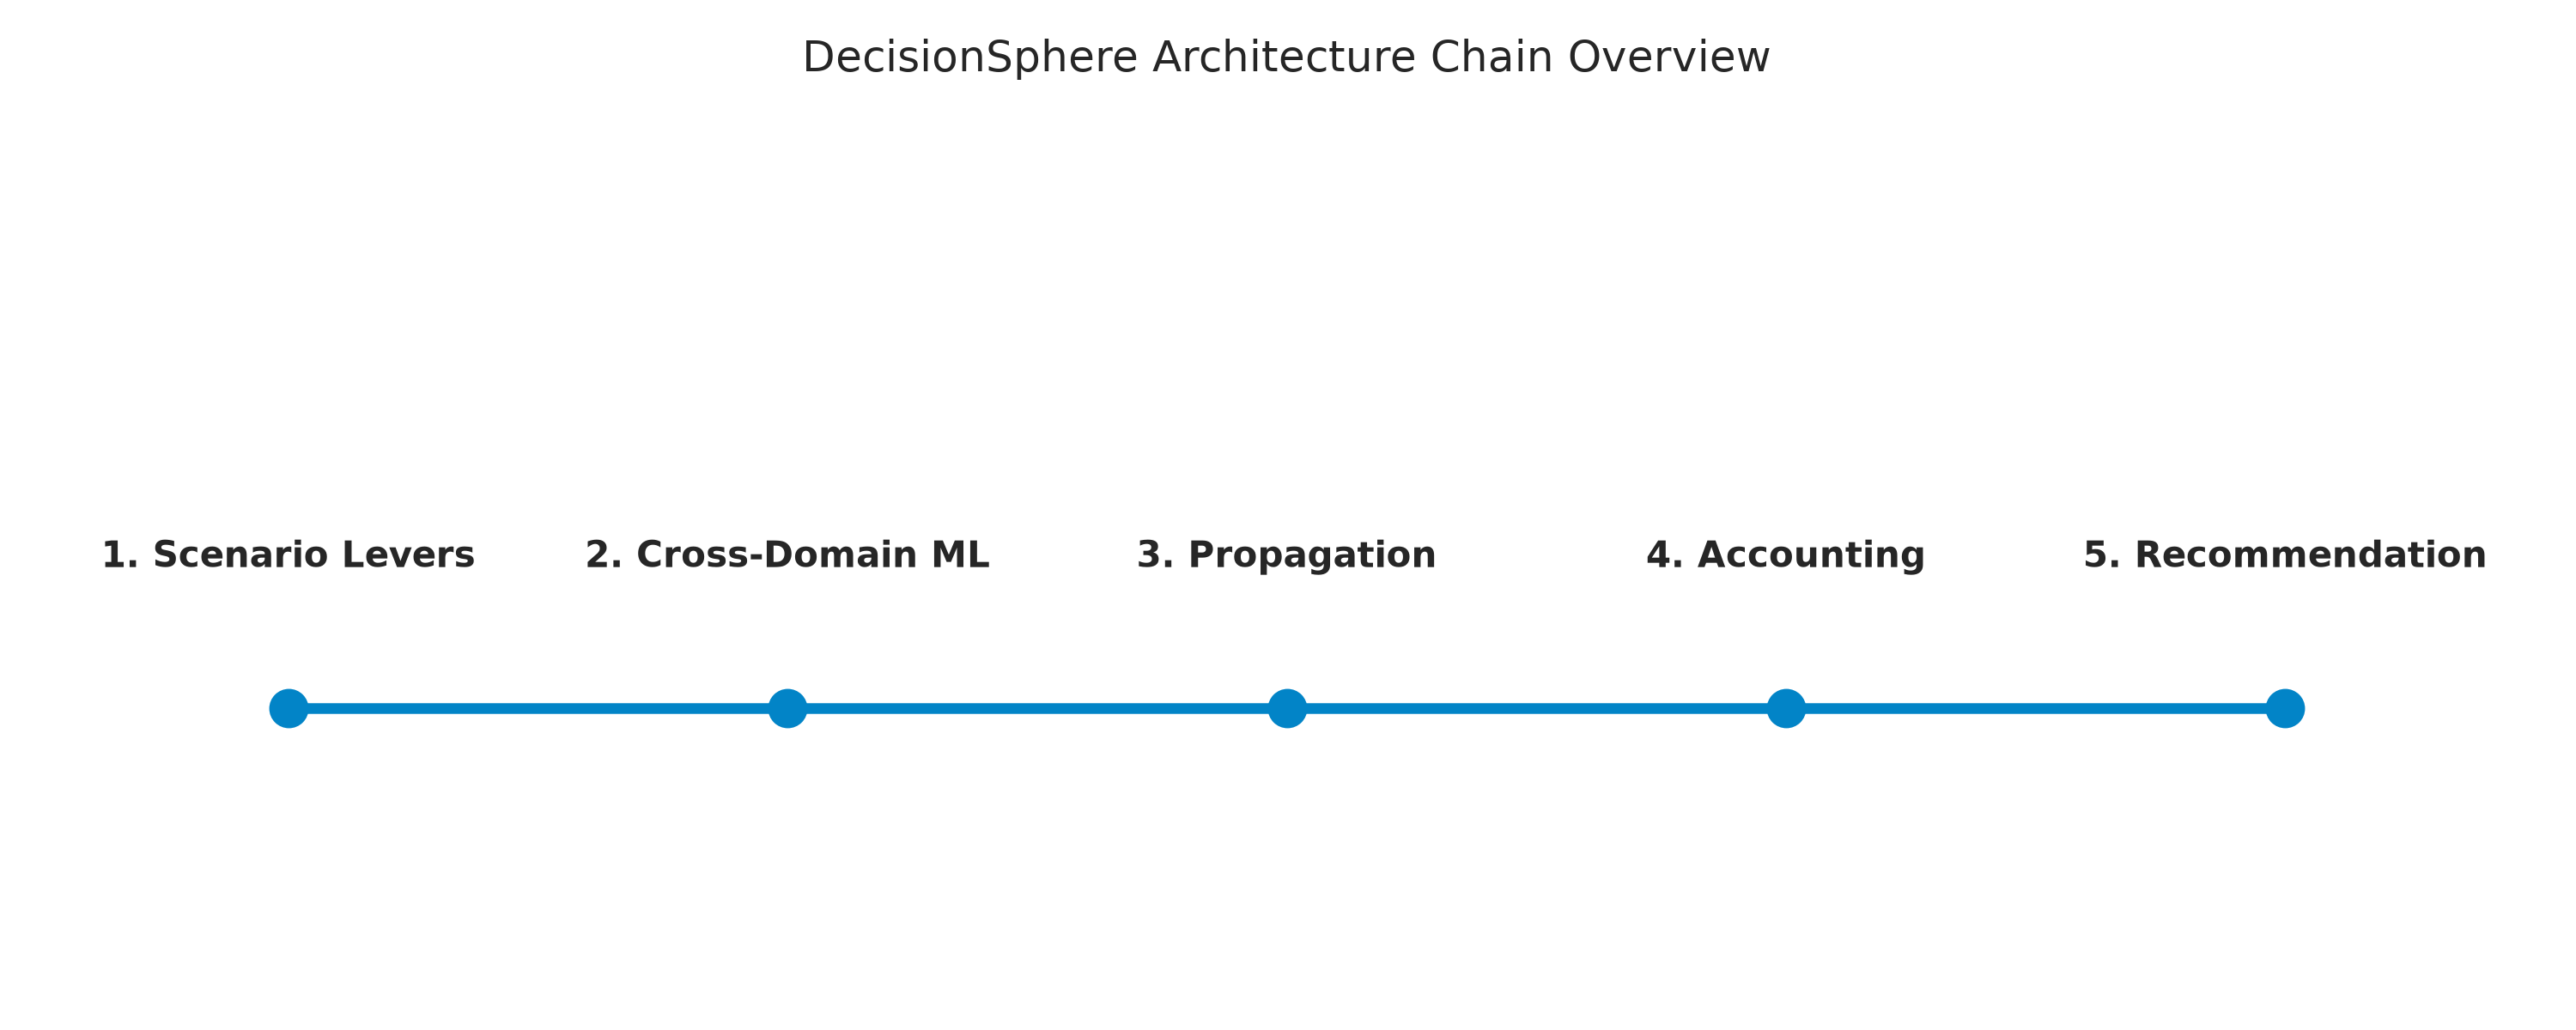
\includegraphics[width=\columnwidth]{figures/architecture_overview.png}}
\caption{DecisionSphere 13-stage end-to-end execution architecture.}
\label{fig:arch}
\end{figure}

\section{Authoritative Canonical Scenario Evaluation}

To validate system behavior under realistic enterprise conditions, we evaluate the authoritative canonical scenario defined in Table~\ref{tab:canonical_scenario}.

\begin{table}[htbp]
\caption{Authoritative Canonical Review 2 Scenario Parameters}
\begin{center}
\begin{tabular}{llc}
\toprule
\textbf{Parameter} & \textbf{Operational Setting} & \textbf{Value} \\
\midrule
Demand Shock ($\Delta D$) & Commercial promotional push & $+15.0\%$ \\
Promotion Status ($P$) & Marketing campaign active & Active \\
Lead Time Offset ($\Delta L$) & Contractual SLA tolerance & $0\text{ days}$ \\
Shipping Mode ($M_{\text{ship}}$) & Default logistics tier & Standard Class \\
Mandatory Overtime ($\Delta O$) & Capacity expansion schedule & $40.0\%$ \\
Salary Adjustment ($\Delta W$) & Baseline wage compensation & None ($0.0\%$) \\
\bottomrule
\end{tabular}
\label{tab:canonical_scenario}
\end{center}
\end{table}

\subsection{Empirical Results}
Executing the canonical scenario across the live analytical core produces exact, verified metrics:
\begin{itemize}
    \item \textbf{Demand Forecast:} Baseline $55,666.31$ units $\to$ Scenario $84,217.35$ units ($\Delta = +28,551.04$ units, $+51.29\%$).
    \item \textbf{Logistics Late Delivery:} Baseline $49.24\% \to$ Scenario $47.11\%$ ($\Delta = -2.13\text{ percentage points}$).
    \item \textbf{Workforce Attrition:} Baseline $16.51\% \to$ Scenario $18.85\%$ ($\Delta = +2.34\text{ percentage points}$).
    \item \textbf{Financial Breakdown (visualized in Fig.~\ref{fig:waterfall}):}
    \begin{itemize}
        \item Gross Revenue Delta: $+\$28,551.04$
        \item Realized Revenue Delta (Fulfillment Loss): $+\$26,710.78$
        \item Cost of Goods Sold (COGS) Delta: $+\$16,026.47$
        \item Logistics Disruption Cost Delta: $+\$469,188.49$
        \item Workforce Overtime \& Turnover Cost: $+\$184,212.00$
        \item \textbf{Net Operating Profit Delta ($\Delta \Pi$): $-\$642,716.18$}
    \end{itemize}
    \item \textbf{Risk Assessment:} Composite Risk Score $\text{CRS} = 37.48 / 100$ (\texttt{MODERATE RISK}).
    \item \textbf{Strategic Synthesis:} Decision category \texttt{REJECT\_RESTRUCTURE}, automatically triggering \texttt{[RULE-04] ACT-FIN-001: Margin Erosion Warning}.
\end{itemize}

\begin{figure}[htbp]
\centerline{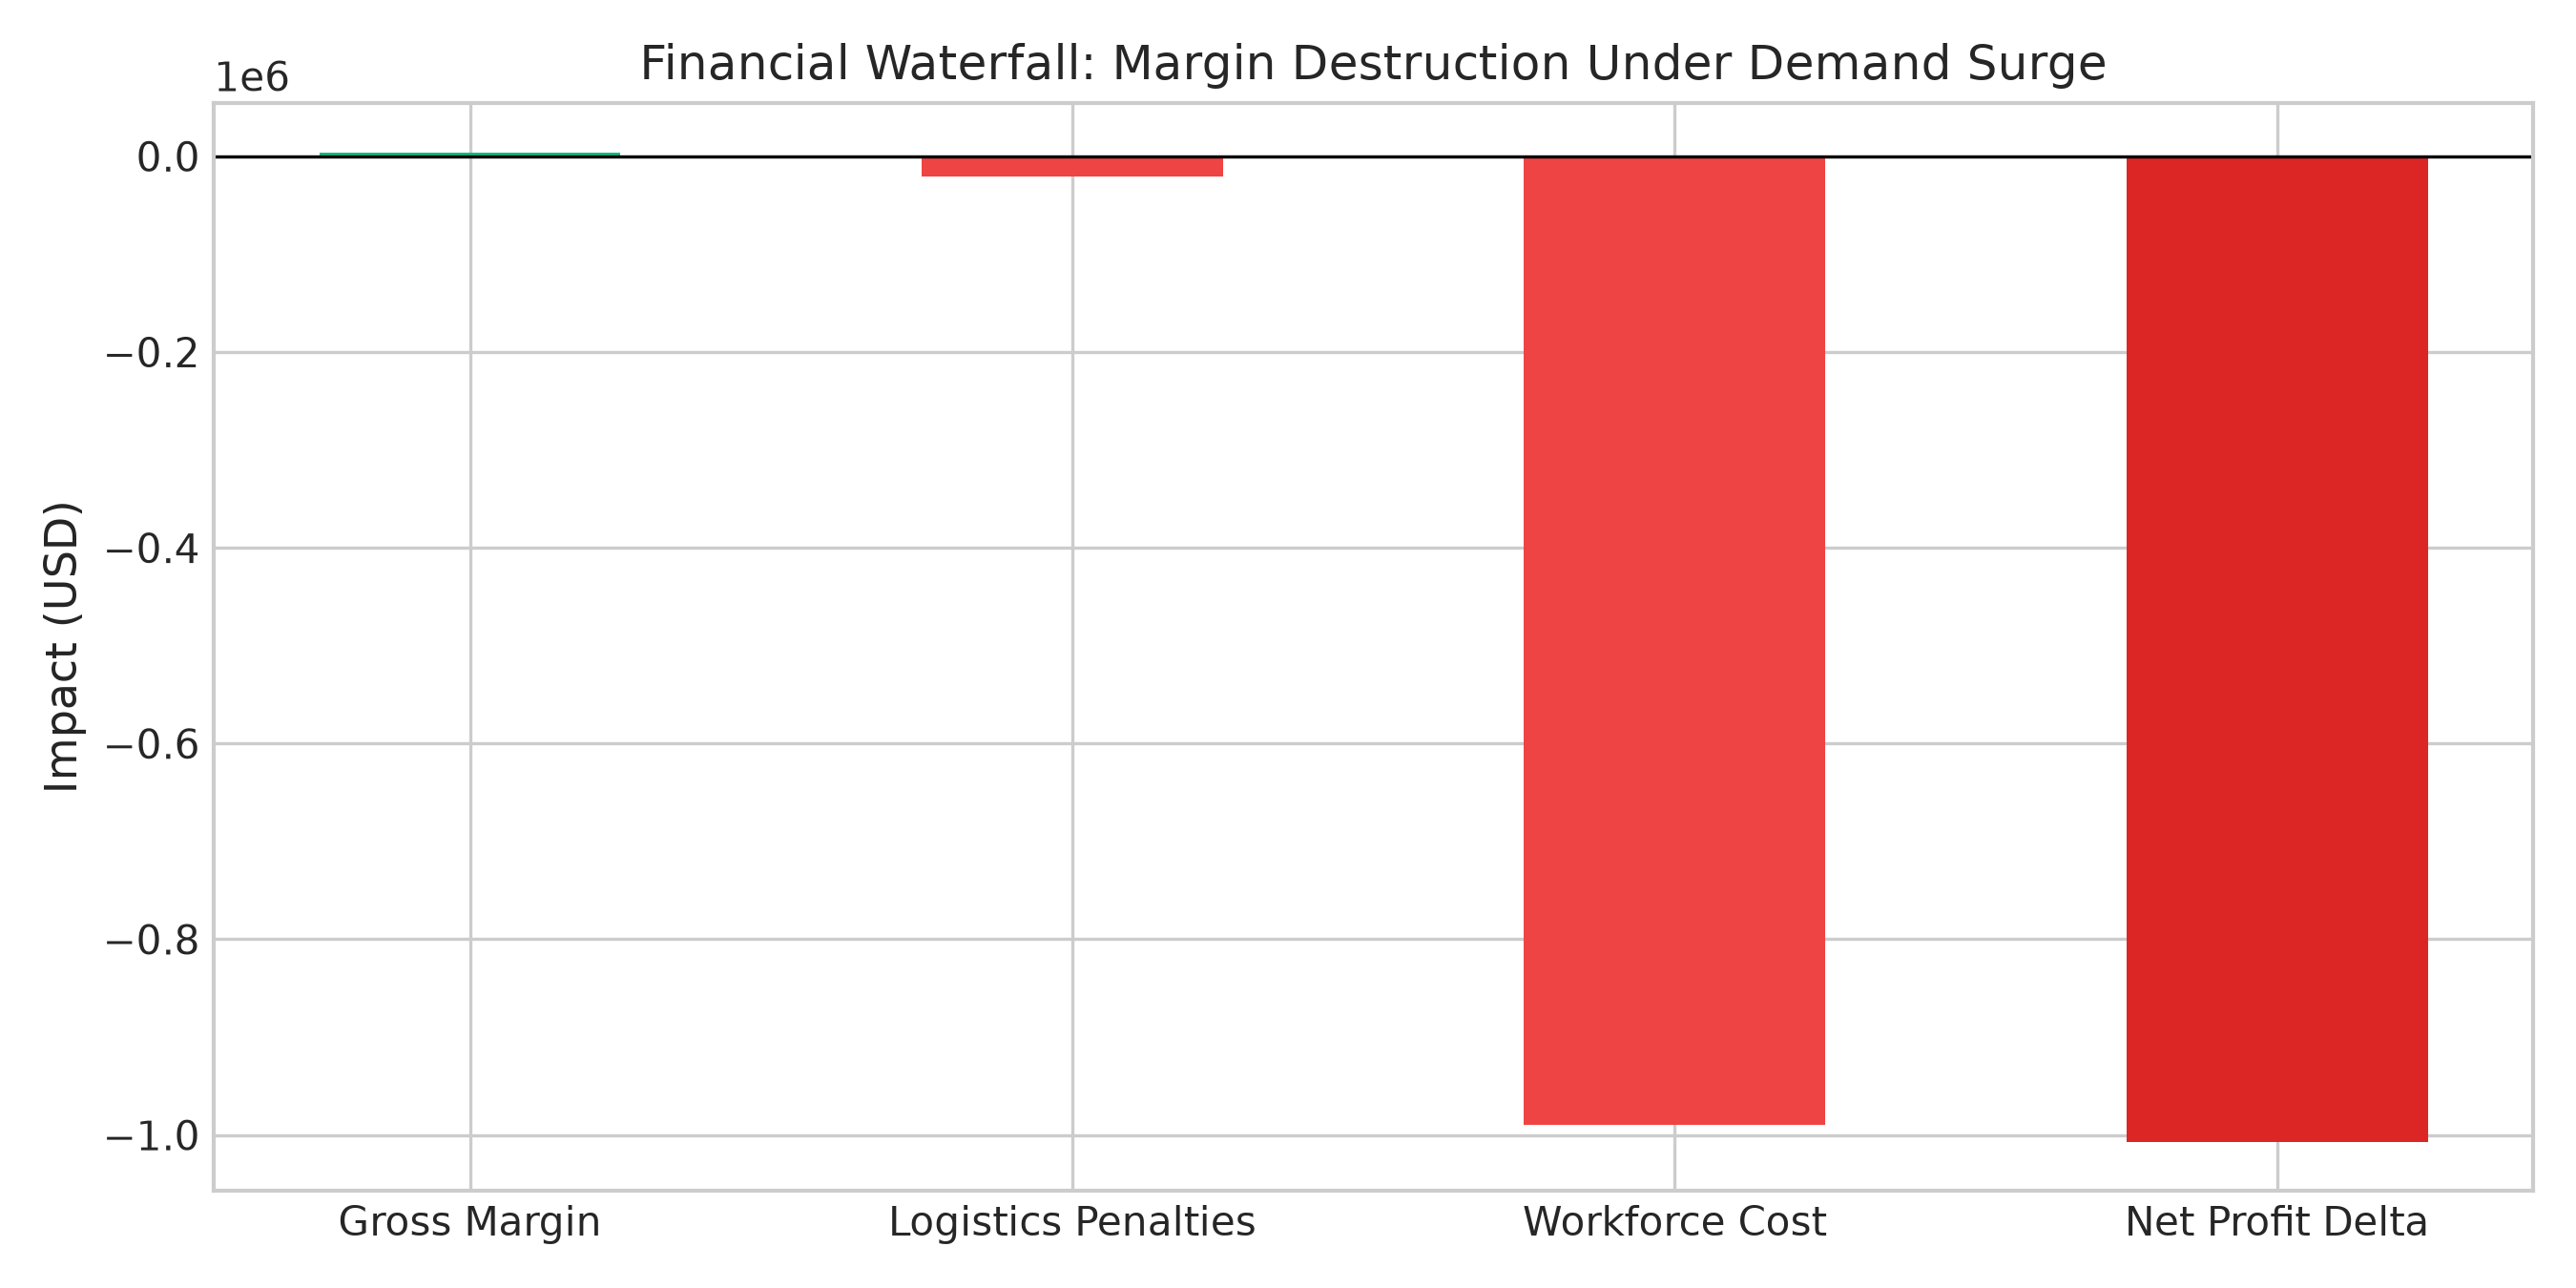
\includegraphics[width=\columnwidth]{figures/financial_waterfall.png}}
\caption{Managerial accounting financial waterfall for canonical scenario.}
\label{fig:waterfall}
\end{figure}

\subsection{Multidimensional Sensitivity Analysis}
Unidimensional sweeps across delay penalties (\$10--\$60/order) and overtime multipliers reveal that profitability collapses into negative territory when promotional demand surges exceed $+12.5\%$ under standard shipping logistics. Tipping point analysis confirms that unbuffered promotions inherently destroy value unless accompanied by dedicated carrier capacity reservations.

\section{Discussion}

\subsection{The Growth Paradox}
The canonical scenario demonstrates an empirical phenomenon we define as the \textit{Operational Growth Paradox}: rapid commercial expansion without concurrent operational buffering destroys enterprise value. Because logistics networks and human workforces exhibit inelastic short-term capacity, non-linear overtime wage premiums and carrier penalty schedules rapidly outpace marginal gross revenues.

\subsection{Epistemic Demarcation and Non-Causality}
In accordance with Shmueli's epistemological framework \cite{shmueli2010explain}, we explicitly reiterate that DecisionSphere models predictive associations ($P(Y \mid X)$), not causal effects. TreeSHAP values prove feature attribution within frozen mathematical estimators, not physical causation. By maintaining clear boundaries between observed data, predictive inferences, and assumed coupling dynamics, DecisionSphere provides auditable decision guidance without ungrounded scientific claims.

\section{Limitations and Threats to Validity}

Several threats to validity must be disclosed:
\begin{enumerate}
    \item \textbf{Benchmark Generalization:} The platform is calibrated on public benchmarks (Rossmann, DataCo, IBM HR). While these datasets represent realistic industrial distributions, cross-domain coupling parameters are modeled as parameterized assumptions ($\mathbf{c}_{\text{cost}}$).
    \item \textbf{Observational Non-Causality:} The system assumes operational feature invariance outside declared scenario levers. Unmodeled macroeconomic shocks or competitor reactions are excluded.
    \item \textbf{Static Cost Schedules:} Penalty and wage schedules are modeled as piecewise linear constants rather than dynamic spot-market auctions.
\end{enumerate}

\section{Reproducibility Protocol}

DecisionSphere guarantees complete academic reproducibility:
\begin{itemize}
    \item All 16 Jupyter notebooks execute sequentially without human intervention.
    \item Serialized models match verified cryptographic SHA-256 digests:
    \begin{itemize}
        \item Demand: \texttt{fb438c03a742202657bb4ef9196ff17e004bc090e99218f02985dc7720f41941}
        \item Supply Chain: \texttt{0052e641cf355257abb332703c3e6a46c65e9ab10a975227d83cf77d7e689b59}
        \item Workforce: \texttt{4b195c7bee3ab8f4afe75ccd0c75fff0c8e18b9fca88a00305e165a010109918}
    \end{itemize}
    \item The test suite executes 236 automated unit and integration tests across core, backend, and frontend environments with zero failures.
\end{itemize}

\section{Conclusion}

This paper presented DecisionSphere, an integrated scenario-based strategic planning and risk evaluation platform. By synthesizing retail demand forecasting, supply chain delivery risk, and workforce attrition modeling into a coupled 13-stage pipeline with deterministic managerial accounting, DecisionSphere resolves the operational silos that hinder modern enterprise decision support. Our empirical evaluation of an unbuffered commercial promotion demonstrates how uncoordinated demand shocks precipitate a $-\$642,716.18$ net profit collapse, automatically caught by objective rule-grounded governance. DecisionSphere provides a reproducible, auditable blueprint for next-generation enterprise decision intelligence.

\bibliographystyle{IEEEtran}
\bibliography{references}

\end{document}
